% !TEX root = ../report.tex
\chapter{Конструкторская часть}
\section{Требования к программе}
Программа должна обеспечивать ввод размера массива и его элементов, сохранение исходного массива и подготовку отсортированной копии. При вводе размера, равного нулю, используется массив по умолчанию из десяти нечётных положительных чисел.

Программа служит испытательным стендом для сравнения алгоритмов. После подготовки данных она должна выводить меню и принимать искомое значение. В меню выбирается отдельный алгоритм или режим сравнения всех четырёх алгоритмов. Результатом поиска является индекс либо сообщение об отсутствии элемента. Для выбранного алгоритма указывается, к какому массиву относится индекс. Режим сравнения должен выводить индекс и число сравнений для каждого алгоритма.

Основные функции поиска должны возвращать только индекс. Расширенные функции для исследования должны дополнительно возвращать число выполненных сравнений искомого значения с элементами массива.

\section{Структура программы}
Программа состоит из модуля подготовки массивов, четырёх модулей алгоритмов поиска, модуля меню, диспетчера и точки входа. Функция \texttt{main} создаёт и освобождает исходный массив и его отсортированную копию. Диспетчер передаёт оба массива модулю меню. Для линейного поиска выбирается исходный массив, для остальных алгоритмов --- отсортированная копия.

Каждая функция поиска получает указатель на массив, его размер и искомое значение. Функции поиска не меняют значения элементов и их порядок. Для бинарного поиска требуется неубывающий порядок. Расширенная функция возвращает структуру с полями \texttt{index} и \texttt{comparisons}.

\section{Схемы алгоритмов}
В схемах используются имена параметров и переменных из исходного кода: \texttt{arr} --- массив, \texttt{size} --- его размер, \texttt{standart} --- искомое значение. Деление целочисленное. Функция \texttt{compare(a, b)} возвращает результат сравнения $a<b$. В составных условиях вторая часть проверяется только тогда, когда первая истинна. Рекурсивная функция возвращает индекс относительно переданного подмассива; при поиске в правой части к нему прибавляется \texttt{median + 1}.

% !TEX root = ../report.tex
Схема линейного поиска представлена на рисунке~\ref{fig:linear}.

\begin{figure}[H]
\centering
\begin{tikzpicture}[flow]
\node[term] (start) at (0,0.0) {Начало: $a,N,x$};
\node[proc] (init) at (0,-1.6) {$i\gets0$};
\node[decision] (loop) at (0,-3.9) {$i<N$};
\node[decision] (equal) at (0,-6.7) {$a_i=x$};
\node[proc] (inc) at (0,-9.0) {$i\gets i+1$};
\node[term] (miss) at (5,-3.9) {Возврат $-1$};
\node[term] (found) at (5,-6.7) {Возврат $i$};
\draw[arrow] (start)--(init);
\draw[arrow] (init)--(loop);
\draw[arrow] (loop)--node[left]{Да}(equal);
\draw[arrow] (loop)--node[above]{Нет}(miss);
\draw[arrow] (equal)--node[above]{Да}(found);
\draw[arrow] (equal)--node[left]{Нет}(inc);
\draw[arrow] (inc.west)--(-3,-9.0)--(-3,-2.5)--(0,-2.5)--(loop.north);
\end{tikzpicture}
\caption{Схема линейного поиска}\label{fig:linear}
\end{figure}

% !TEX root = ../report.tex
\clearpage
Схема классического нерекурсивного бинарного поиска представлена на рисунке~\ref{fig:classic}.

\begin{figure}[H]
\centering
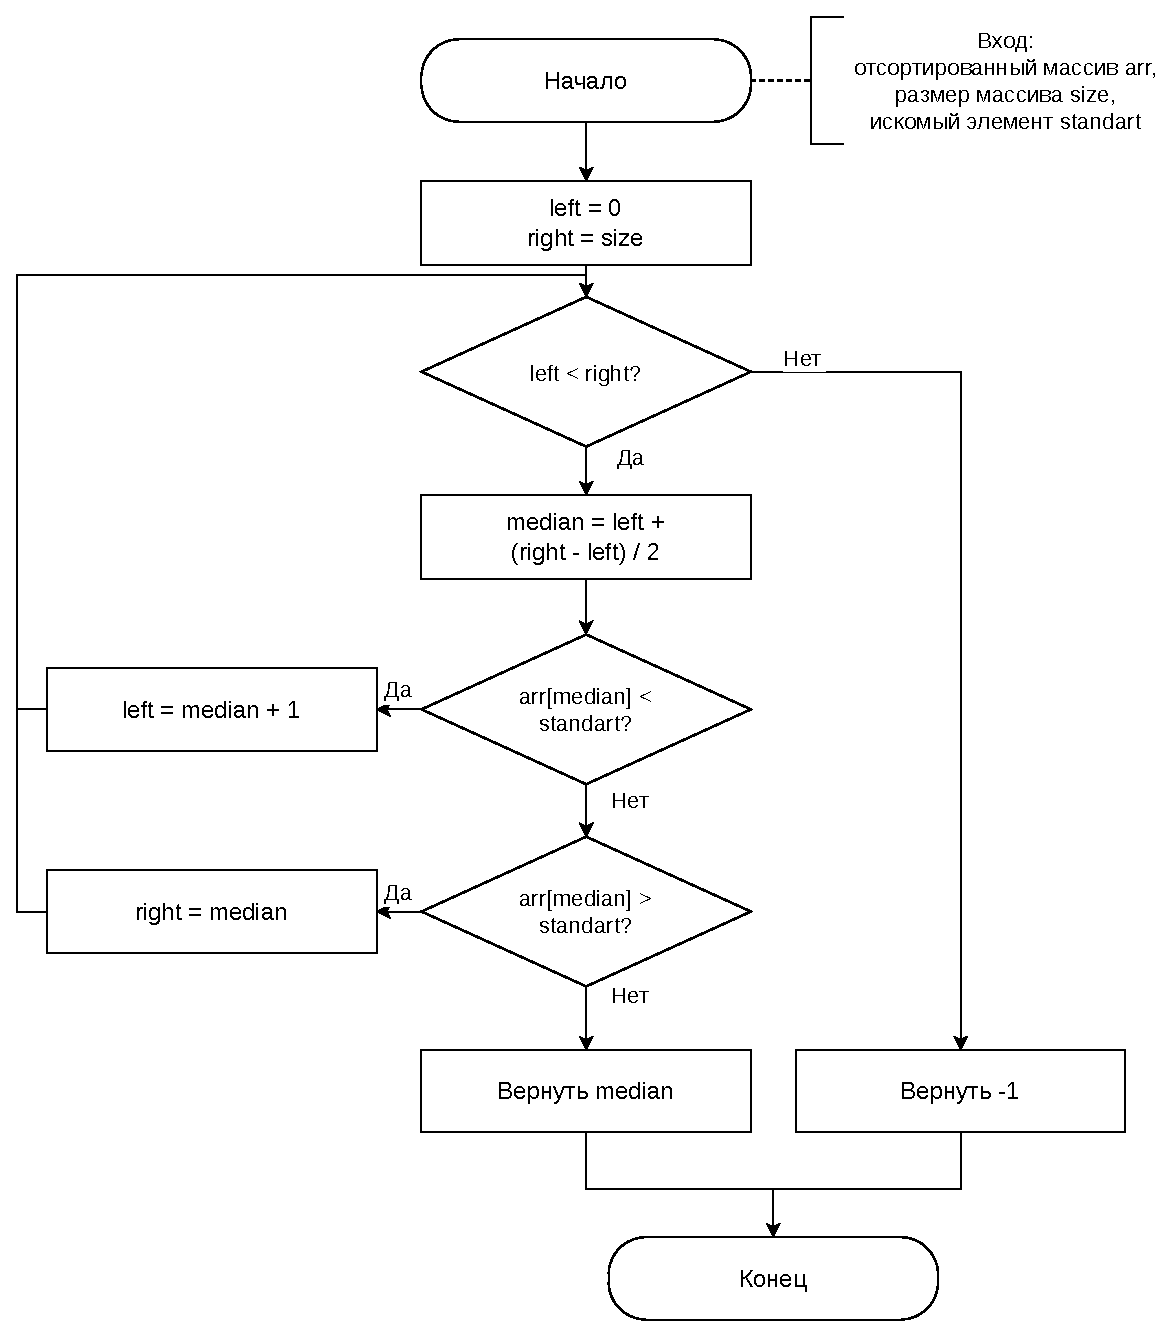
\includegraphics[width=\linewidth,height=0.86\textheight,keepaspectratio]{figures/classic_report.pdf}
\caption{Схема классического нерекурсивного бинарного поиска}\label{fig:classic}
\end{figure}

% !TEX root = ../report.tex
\clearpage
Схема бинарного поиска без ветвления представлена на рисунке~\ref{fig:branchless}.

\begin{figure}[H]
\centering
\begin{tikzpicture}[flow]
\node[term] (start) at (0,0) {Начало: $a,N,x$};
\node[decision] (empty) at (0,-2.1) {$N=0$};
\node[term] (emptyret) at (5.1,-2.1) {Возврат $-1$};
\node[proc] (init) at (0,-4.2) {$b\gets0$, $e\gets N$\\$s\gets\texttt{bit\_floor}(N)$};
\node[decision] (prepare) at (0,-6.7) {$s\ne N$ и\\$a_s<x$};
\node[proc] (tail) at (0,-9) {$e\gets e-s-1$};
\node[decision] (zero) at (0,-11.3) {$e=0$};
\node[term] (earlyret) at (5.1,-11.3) {Возврат $-1$};
\node[proc] (restart) at (0,-13.6) {$s\gets\texttt{bit\_ceil}(e)$\\$b\gets N-s$};
\node[proc] (halve) at (0,-15.7) {$s\gets s/2$};
\node[decision] (loop) at (0,-17.8) {$s\ne0$};
\node[decision] (compare) at (0,-20.3) {$a_{b+s}<x$};
\node[proc] (advance) at (0,-22.6) {$b\gets b+s$};
\node[proc] (candidate) at (5.1,-17.8) {$i\gets b+$\\$\texttt{compare}(a_b,x)$};
\node[decision] (equal) at (5.1,-20.3) {$i<N$ и\\$a_i=x$};
\node[term] (found) at (5.1,-22.6) {Возврат $i$};
\node[term] (miss) at (10.0,-22.6) {Возврат $-1$};
\draw[arrow] (start)--(empty);
\draw[arrow] (empty)--node[above]{Да}(emptyret);
\draw[arrow] (empty)--node[left]{Нет}(init);
\draw[arrow] (init)--(prepare);
\draw[arrow] (prepare)--node[left]{Да}(tail);
\draw[arrow] (prepare.west)--node[above]{Нет}(-3.7,-6.7)--(-3.7,-14.9)--(0,-14.9)--(halve.north);
\draw[arrow] (tail)--(zero);
\draw[arrow] (zero)--node[above]{Да}(earlyret);
\draw[arrow] (zero)--node[left]{Нет}(restart);
\draw[arrow] (restart)--(halve);
\draw[arrow] (halve)--(loop);
\draw[arrow] (loop)--node[left]{Да}(compare);
\draw[arrow] (loop)--node[above]{Нет}(candidate);
\draw[arrow] (compare)--node[left]{Да}(advance);
\draw[arrow] (compare.west)--node[above]{Нет}(-3.7,-20.3)--(-3.7,-15.7)--(halve.west);
\draw[arrow] (advance.west)--(-4.3,-22.6)--(-4.3,-15.7)--(halve.west);
\draw[arrow] (candidate)--(equal);
\draw[arrow] (equal)--node[left]{Да}(found);
\draw[arrow] (equal.east)--node[above]{Нет}(10.0,-20.3)--(miss.north);
\end{tikzpicture}
\caption{Схема бинарного поиска без ветвления}\label{fig:branchless}
\end{figure}

% !TEX root = ../report.tex
\clearpage
Схема рекурсивного бинарного поиска представлена на рисунке~\ref{fig:recursive}.

\begin{figure}[H]
\centering
\begin{tikzpicture}[flow]
\node[term] (start) at (0,0.0) {Начало: $a,N,x$};
\node[decision] (empty) at (0,-2.1) {$N=0$};
\node[term] (miss) at (4.8,-2.1) {Возврат $-1$};
\node[proc] (mid) at (0,-4.4) {$M\gets\lfloor N/2\rfloor$};
\node[decision] (equal) at (0,-6.7) {$a_M=x$};
\node[term] (found) at (4.8,-6.7) {Возврат $M$};
\node[decision] (lt) at (0,-9.5) {$a_M<x$};
\node[proc] (lcall) at (-3.2,-12.0) {$q\gets\mathrm{B}(a,M,x)$};
\node[proc] (rcall) at (3.2,-12.0) {$q\gets\mathrm{B}(a+M+1,$\\$N-M-1,x)$};
\foreach \n in {lcall,rcall} {
\draw ([xshift=2mm]\n.south west)--([xshift=2mm]\n.north west);
\draw ([xshift=-2mm]\n.south east)--([xshift=-2mm]\n.north east);
}
\node[term] (lret) at (-3.2,-14.5) {Возврат $q$};
\node[decision] (qmiss) at (3.2,-14.5) {$q=-1$};
\node[term] (rmiss) at (6.2,-17.0) {Возврат $-1$};
\node[term] (rret) at (1.7,-17.0) {Возврат $M+1+q$};
\draw[arrow] (start)--(empty);
\draw[arrow] (empty)--node[above]{Да}(miss);
\draw[arrow] (empty)--node[left]{Нет}(mid);
\draw[arrow] (mid)--(equal);
\draw[arrow] (equal)--node[above]{Да}(found);
\draw[arrow] (equal)--node[left]{Нет}(lt);
\draw[arrow] (lt.west)-|node[above,near start]{Нет}(lcall.north);
\draw[arrow] (lt.east)-|node[above,near start]{Да}(rcall.north);
\draw[arrow] (lcall)--(lret);
\draw[arrow] (rcall)--(qmiss);
\draw[arrow] (qmiss.east)-|node[above,near start]{Да}(rmiss.north);
\draw[arrow] (qmiss.south)|-node[above,near end]{Нет}(1.7,-16.0)--(rret.north);
\end{tikzpicture}
\caption{Схема рекурсивного бинарного поиска}\label{fig:recursive}
\end{figure}

\clearpage
\section*{Вывод}
Разработаны схемы четырёх функций поиска. Для сравнения алгоритмов предусмотрены отдельные версии функций, которые дополнительно подсчитывают число сравнений.
